\hypertarget{pro3d.gis}{%
\subsection{PRo3D.GIS}\label{pro3d.gis}}

Summary: This feature allows to interpret celestial bodies and surfaces
from within pro3d and serves as a basis for GIS functionality in PRo3D.
General concept: A new UI tab allows to assign coordiante frames and
celestial body information to surfaces and GIS entities. By setting
observeration time and by choosing an observer body, views or fly-by
scenarious can be modelled.

\hypertarget{spice}{%
\subsection{SPICE}\label{spice}}

\hypertarget{pre-requisistes}{%
\subsubsection{Pre-requisistes}\label{pre-requisistes}}

As mentioned in \href{./spice.md}{SPICE docs} pro3d allows to load
custom spice kernels. In this documentation we use the
\href{https://s2e2.cosmos.esa.int/bitbucket/projects/spice_kernels/repos/hera/browse}{HERA
spice kernels}, which are also used in the
\href{https://github.com/pro3d-space/PRo3D.SPICE}{solar-system demo}

To follow the demo download or clone the
\href{https://s2e2.cosmos.esa.int/bitbucket/projects/spice_kernels/repos/hera/browse}{repository}.

\hypertarget{loading-the-kernel}{%
\subsubsection{Loading the kernel}\label{loading-the-kernel}}

There are two options to load SPICE kernels.

\hypertarget{the-command-line}{%
\paragraph{The command line}\label{the-command-line}}

\begin{itemize}
\tightlist
\item
  by using the command-line argument
  \texttt{-\/-defaultSpiceKernel\ path}, e.g.~the path to the tm file:
  \texttt{"../hera/kernels/mk/hera\_crema\_2\_0\_LPC\_ECP\_PDP.tm"}, the
  SPICE kernel to be loaded at application startup can be specified.
\end{itemize}

\hypertarget{the-ui}{%
\paragraph{The UI}\label{the-ui}}

\begin{enumerate}
\def\labelenumi{\arabic{enumi}.}
\tightlist
\item
  Initially PRo3D with GIS view enabled looks like this:
\end{enumerate}

\begin{figure}
\centering
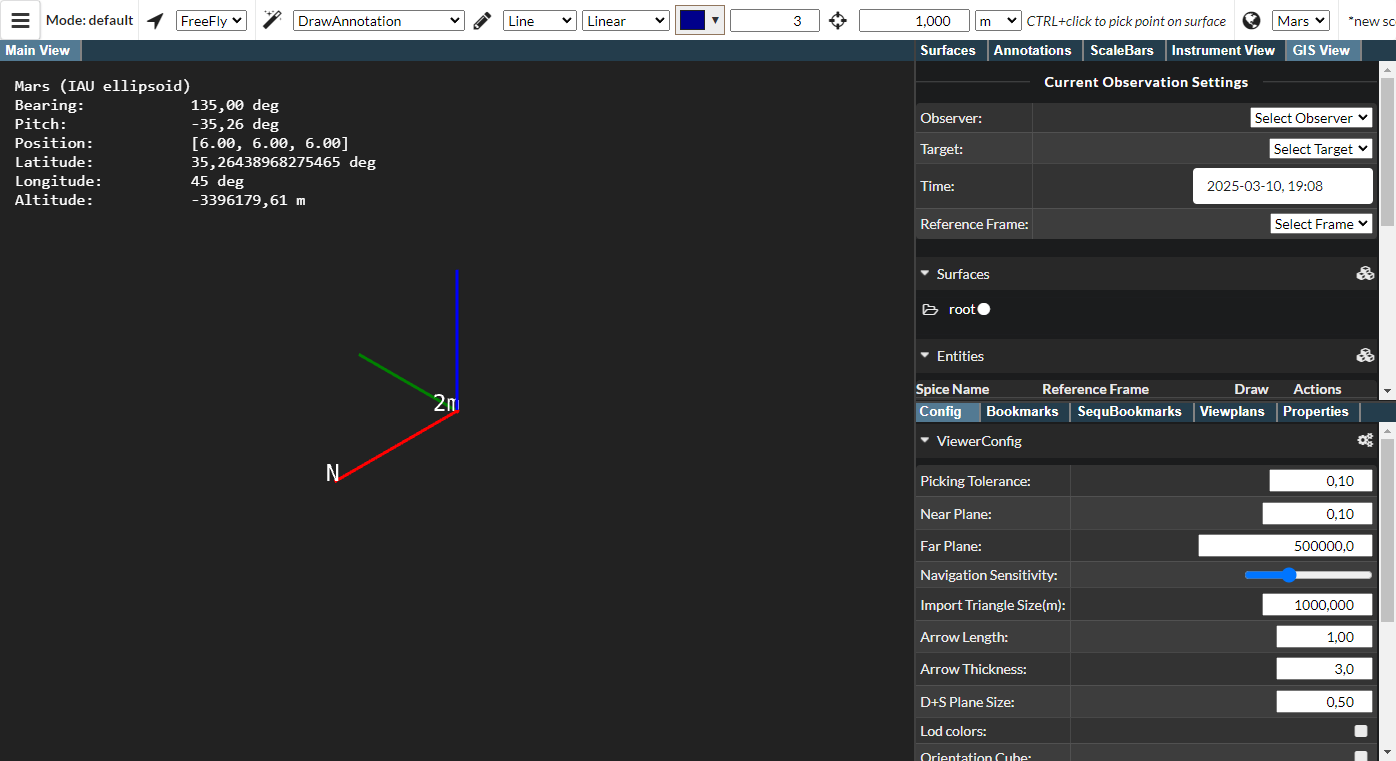
\includegraphics{./images/gis-view.png}
\caption{alt text}
\end{figure}

\begin{enumerate}
\def\labelenumi{\arabic{enumi}.}
\setcounter{enumi}{1}
\tightlist
\item
  Load the kernel via:
\end{enumerate}

\begin{figure}
\centering
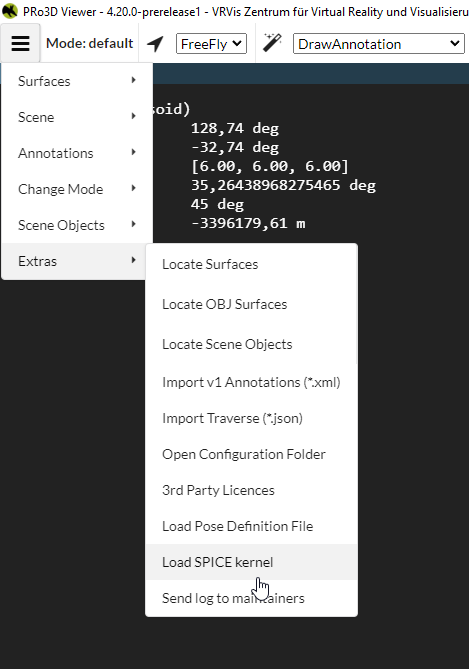
\includegraphics{images/loadKernel.png}
\caption{alt text}
\end{figure}

\begin{enumerate}
\def\labelenumi{\arabic{enumi}.}
\setcounter{enumi}{2}
\tightlist
\item
  Then the Gis View should print the path to the kernel (scroll down,
  and look at the settings pane within the GIS view):
\end{enumerate}

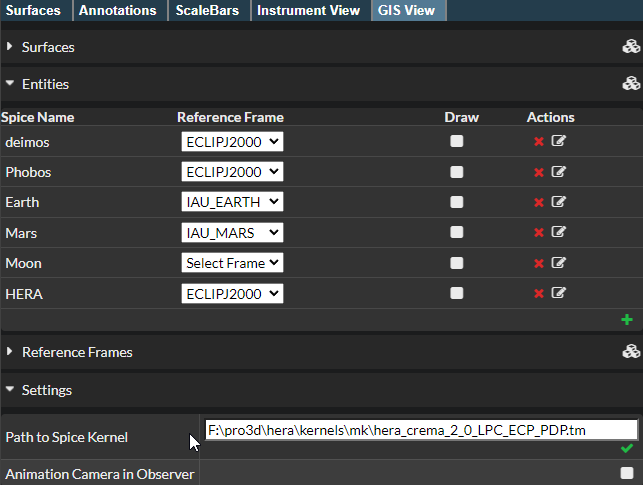
\includegraphics{images/loadedKernel.png}

A green check mark appears below the path if loading the kernel was
successful. If there is a red exclamation mark beneath the path loading
was not successful. PRo3D's text output will give more detailed
information why, it might be that the path to the kernel is not correct.

\hypertarget{pro3d-gis-view-tab}{%
\subsection{PRO3D GIS View Tab}\label{pro3d-gis-view-tab}}

\hypertarget{current-observation-settings}{%
\subsubsection{Current Observation
Settings}\label{current-observation-settings}}

At the top of the GIS tab there is a section entitled ``Current
Observation Settings''. This is used to define an observer, a target, a
point in time, and a reference frame.

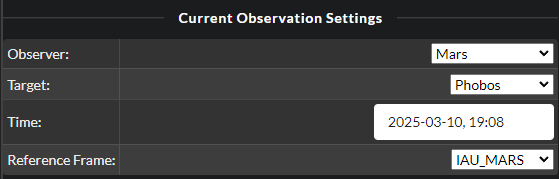
\includegraphics{images/currentObservationSettings.png}

\begin{itemize}
\tightlist
\item
  Observer: The entity from which we want to observe a specific target.
  The camera will be placed at the location of the observer.
\item
  Target: The entity we want to look at. The camera will look in the
  direction of the target.
\item
  Time: The point of time at which we want to observe. The loaded spice
  kernel needs to have data for observer and target at the selected
  point in time!
\item
  Reference Frame: The reference frame into which all other frames will
  be converted. Which frame is selected here should not change the
  visual result.
\end{itemize}

\hypertarget{surfaces}{%
\subsubsection{Surfaces}\label{surfaces}}

To use a surface with PRo3D's GIS functionality, it has to be associated
with a reference frame, and can be associated with an entity. This
reference frame in which the surface is defined is needed to transform
the surface to the global reference system used by PRo3D. Assigning a
reference frame and entity to a loaded surfaces is done in the
``Surfaces'' tab.

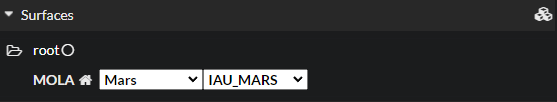
\includegraphics{images/surfaces.png}

Select the correct reference frame (and optionally entity) from the
dropdown menu. If the entity or reference frame needed is not in the
dropdown menu, it can be created in the ``Entities''/``Reference
Frames'' tab.

\hypertarget{entities}{%
\subsubsection{Entities}\label{entities}}

Entities can be celestial bodies or spacecraft. To work with PRO3D's GIS
functionality the Spice Name of the entity needs to be defined in the
loaded spice kernel.

The entity tab lists all entities. There are some default entities
already present in PRo3D.

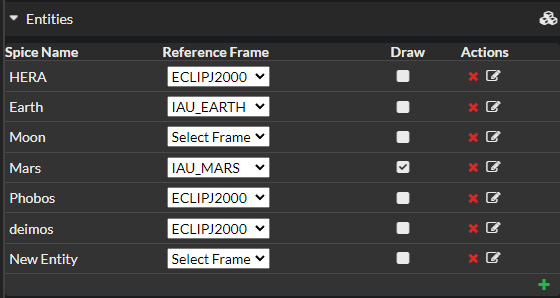
\includegraphics{images/entities.png}

An entity can be edited by clicking on the right hand icon in the
``Actions'' column. The icon used to edit the HERA entity is circled in
red in the screenshot below.

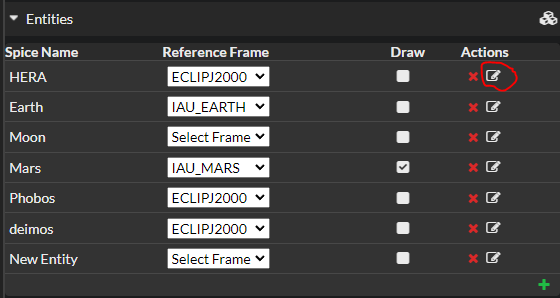
\includegraphics{images/editEntities.png}

The red cross to the left of the edit icon deletes the corresponding
entity.

Each entity can be assigned a reference frame in the column ``Reference
Frame''. For each entity, a sphere can be drawn in the scene. Whether a
sphere is drawn is determined by the checkbox in the ``Draw'' column.

A new entity can be created by clicking on the green plus icon at the
bottom right hand side of the Entities tab. The spice name can only be
set when creating an entity, it cannot be changed once the entity is
created. To change a spice name you need to deleted the old entity and
create a new one with the new spice name and the settings of the old
entity. Spice names are unique, so you cannot create two entities with
the same spice name.

Clicking on the edit icon of an entity (see above), opens a section for
the entity:

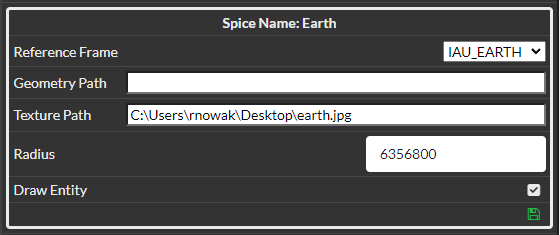
\includegraphics{images/editEntity.png}

The reference frame and whether to draw an entity can be selected in
this view as well as the following settings:

\begin{itemize}
\tightlist
\item
  \textbf{Geometry Path} (not yet implemented) path to a geometry that
  is displayed at the location of this entity instead of a simple sphere
\item
  \textbf{Texture Path} The path to an image (for example a jpeg file)
  that is rendered onto the entity.
\item
  \textbf{Radius} The radius of the sphere that is drawn in the location
  of the entity in meters.
\end{itemize}

The green save icon at the bottom right hand corner closes the edit
view.

Below an example of the entity Moon with a radius of 1736000 meters and
a texture path.

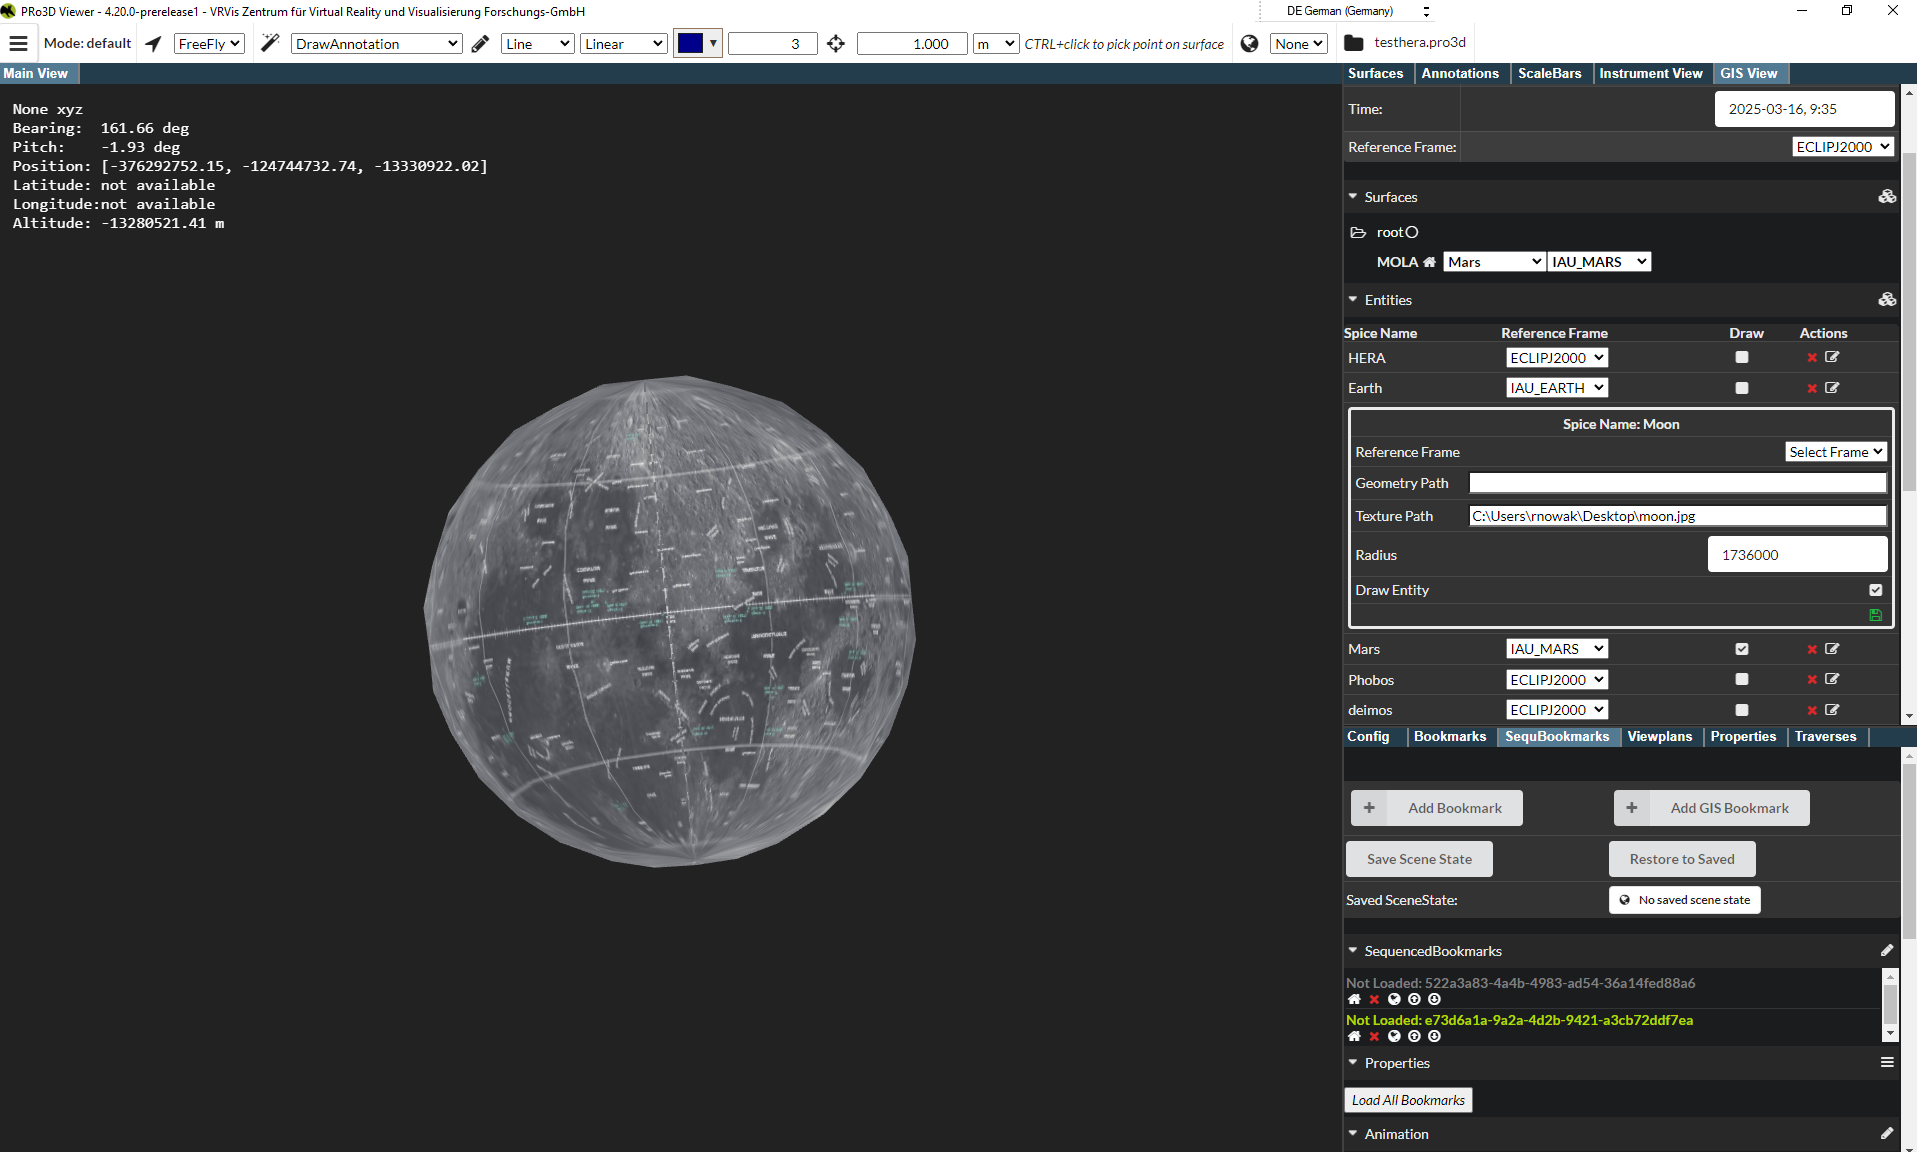
\includegraphics{images/exampleMoonTexture.png}

\hypertarget{reference-frames}{%
\subsection{Reference Frames}\label{reference-frames}}

Reference frames can be deleted (red cross icon) and created (green plus
icon in the bottom right corner) in this view. They can also be assigned
an entity which is associated with them.

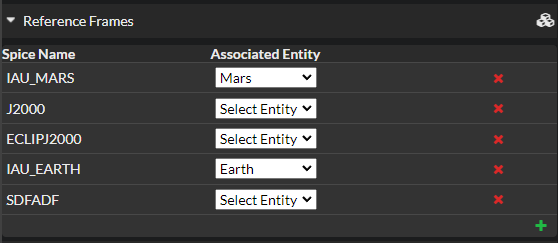
\includegraphics{images/referenceFrames.png}

A new reference frame can be created by clicking on the green plus icon
at the bottom right hand side of the Reference Frames tab. The spice
name can only be set when creating a reference frame, it cannot be
changed once the reference frame is created. To change a spice name you
need to deleted the old reference frame and create a new one with the
new spice name and the settings of the old reference frame. Spice names
are unique, so you cannot create two reference frame with the same spice
name.

\hypertarget{observing-mars}{%
\subsection{Observing mars}\label{observing-mars}}

Let us now observe mars from, say phobos. 1. Set the observation
settings (including a time which is in available in the kernel)
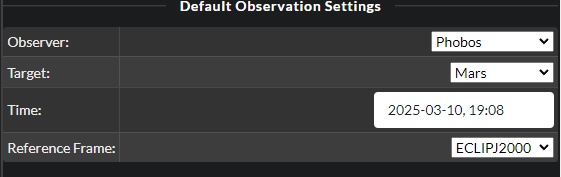
\includegraphics{images/observe.png}

\begin{enumerate}
\def\labelenumi{\arabic{enumi}.}
\setcounter{enumi}{1}
\tightlist
\item
  Next, make sure the proxy visualization for mars is enabled:
  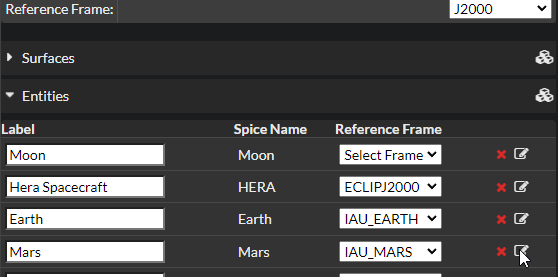
\includegraphics{./images/MarsProperties.png} and
\end{enumerate}

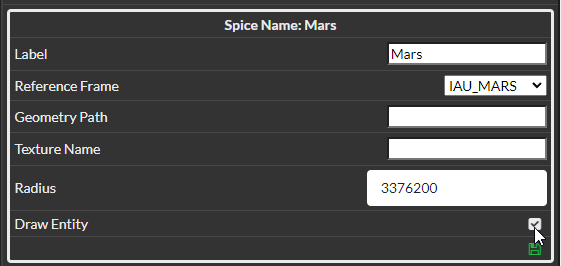
\includegraphics{./images/visibleMars.png}

Also make sure to have the far plane set far away for viewing mars from
phobos. Ajust the near \emph{and} far planes accordingly:
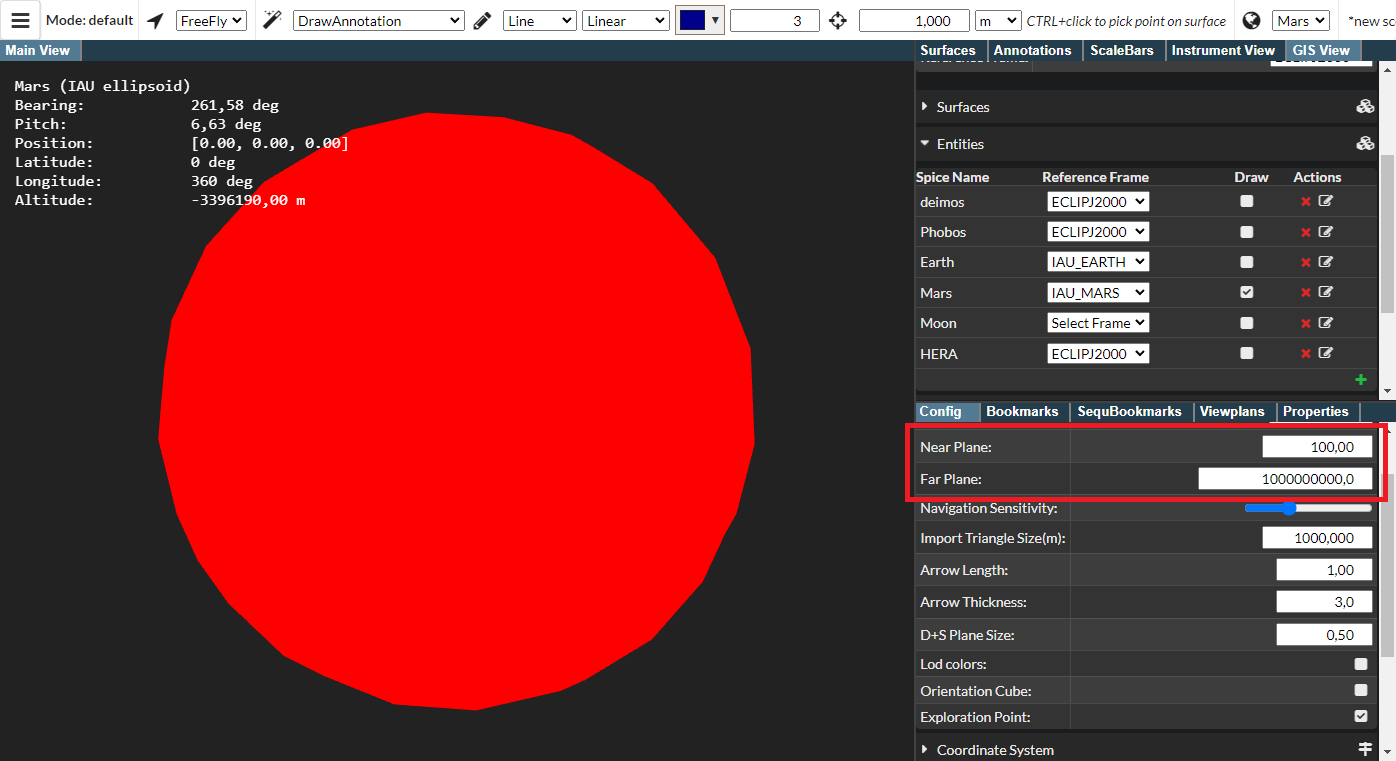
\includegraphics{./images/farplane.png}

Now mars should be visible from the observation point of view.

By using the visualization properties in the entity list the element can
be textured as well.

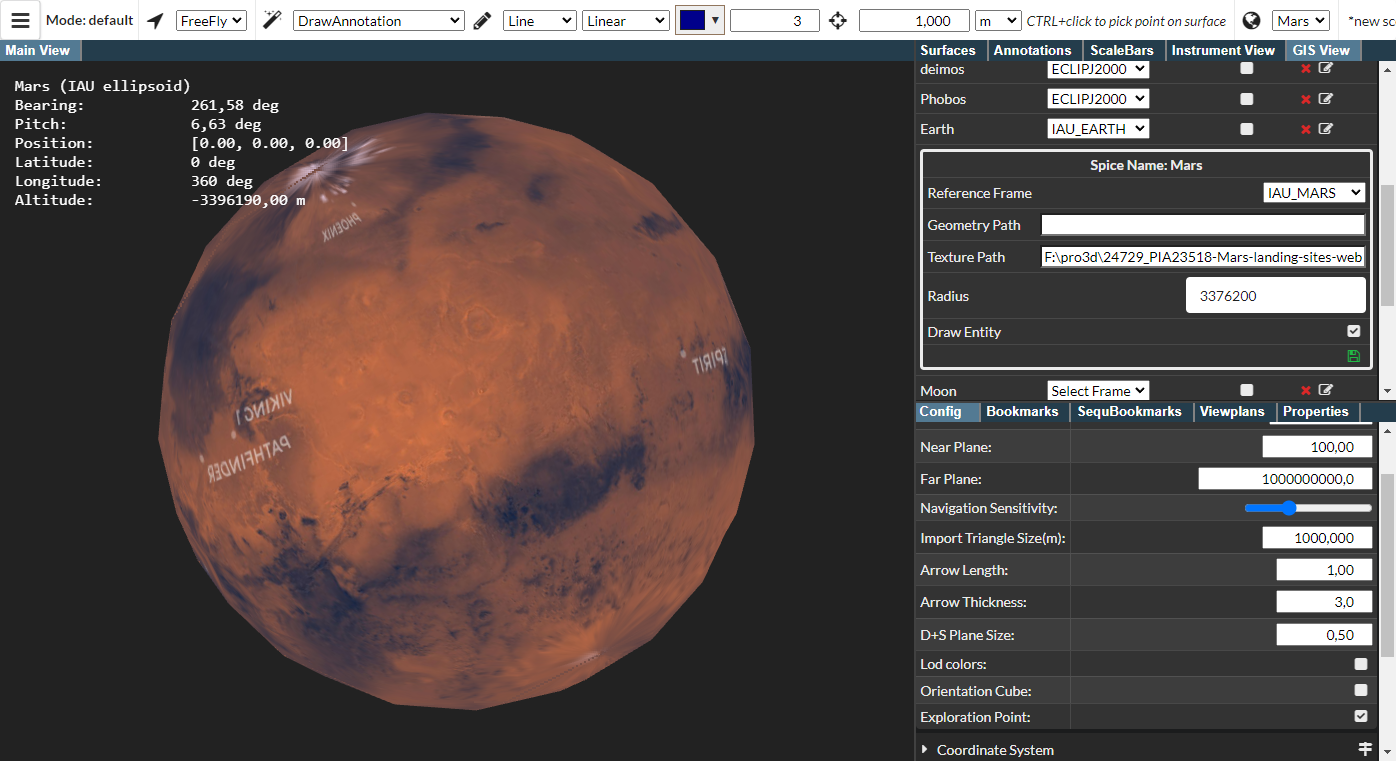
\includegraphics{./images/textured.png}

Next let us load the mola dataset. In the Surfaces pane witin the Gis
View, now specifiy reference frame and celestial body for the surface
(if it does not appear change the observation settings, e.g.~by setting
the time): 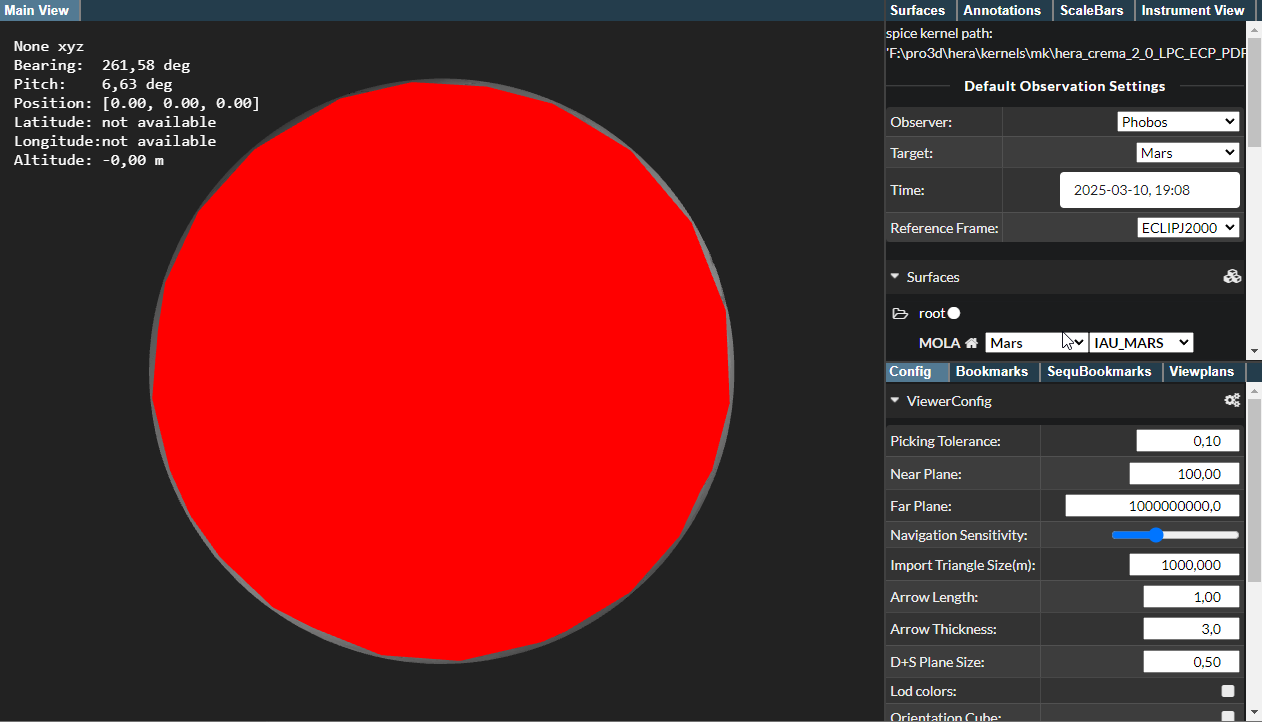
\includegraphics{images/surfaceRefFrame.png}

Since we have a full surface for mars now, we can switch of the proxy
geometry: 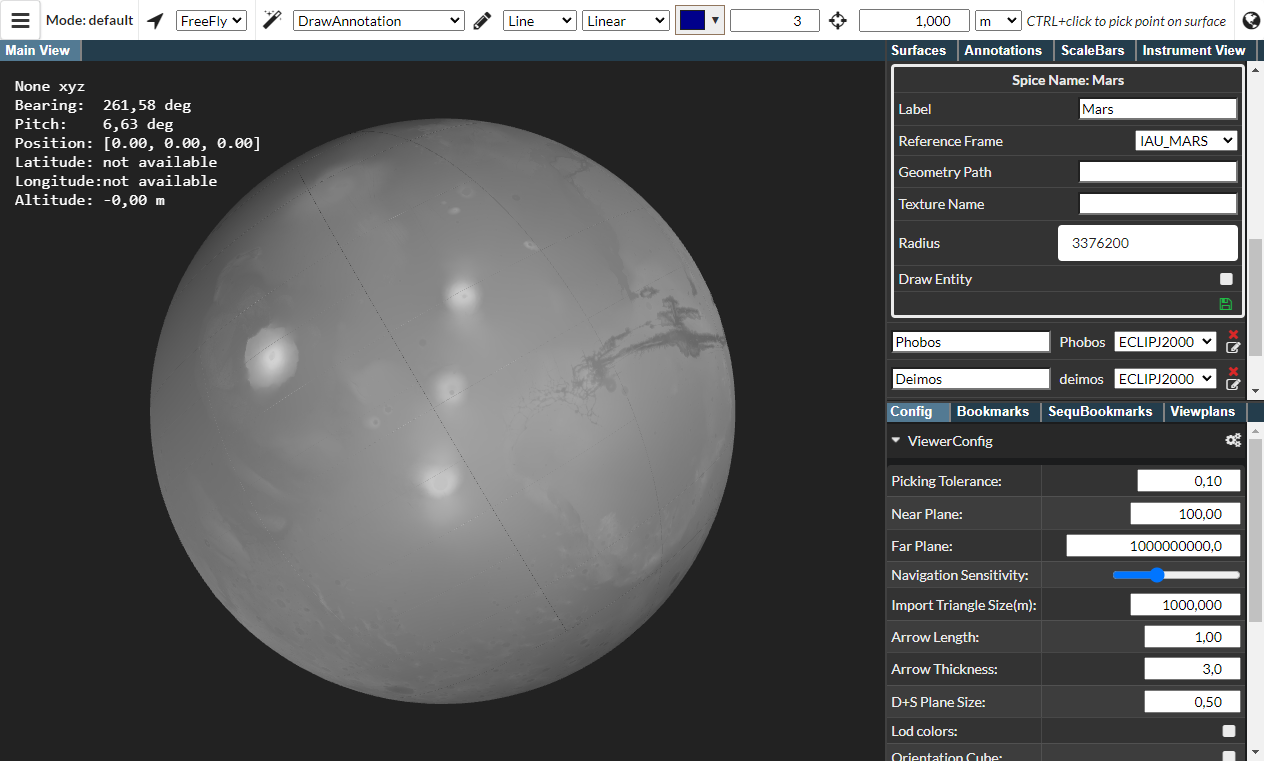
\includegraphics{images/molaObservation.png}

\hypertarget{extended-features}{%
\subsection{Extended features}\label{extended-features}}

It is possible to add new celestial bodies, new reference frames.

\hypertarget{extended-concept}{%
\subsection{Extended concept}\label{extended-concept}}

For story telling, PRo3D also supports to create GIS bookmarks.
Similarly to stories on surfaces this can be used to create movies and
interactive presentations for science.

\hypertarget{caveats}{%
\subsection{Caveats}\label{caveats}}

Currently the GIS settings are not stored to scene files.
